\documentclass[a4paper, 12pt, abstract=on]{scrartcl}
\usepackage[utf8]{inputenc}
\usepackage[T1]{fontenc}
\usepackage{lmodern}

\usepackage[babel=true]{csquotes}
\usepackage[acronym]{glossaries}
\usepackage[english]{babel}
\usepackage{blindtext}

\usepackage{graphicx}
\usepackage{booktabs}
\usepackage{url}
\usepackage{tablefootnote}
\usepackage{hyperref}
\usepackage[per-mode=symbol]{siunitx}
\usepackage{natbib}
\usepackage{floatrow}
\usepackage{pdfpages}

\usepackage{fancyhdr}
\pagestyle{fancy}

% Headers & footers
\lhead{Minesweepers: Towards a Landmine-Free World}
\rhead{}

\newacronym{lipo}{LiPo}{lithium-polymer}
\newacronym{rtt}{RTT}{Round Trip Time}
\newacronym{ekf}{EKF}{Extended Kalman Filter}
\newacronym{imu}{IMU}{Inertial Motion Unit}


\begin{document}

\begin{titlepage}
\begin{center}

\Huge{\textsc{Minesweepers Competition Technical Report}}
\vspace{1cm}~\\
\includegraphics[height=5cm]{emblem}
\vspace{1cm}

\large{\textbf{Club Vaudois de Robotique Autonome (CVRA)}}\\
Switzerland\\
Minesweepers Industry

\vspace{2cm}

\begin{abstract}
    \documentclass[a4paper,twocolumn]{article}

\usepackage[utf8]{inputenc}
\usepackage[T1]{fontenc}
\usepackage[acronym]{glossaries}
\usepackage{graphicx}
\usepackage{fullpage}
\usepackage{booktabs}
\usepackage{hyperref}
\usepackage{listings}
\usepackage{tablefootnote}
\usepackage{verbatim}
\usepackage{multirow}
\usepackage{subcaption}
\usepackage{floatrow}
\usepackage{siunitx}
\usepackage{wasysym}
\usepackage{natbib}
\usepackage{lipsum}
\usepackage{paralist}

\date{July 7, 2017}

\newacronym{gps}{GPS}{Global Positioning System}
\newacronym{imu}{IMU}{Inertial Motion Unit}
\newacronym{uwb}{UWB}{Ultra Wide Band}


\title{Development of an ultra-wide band indoor positioning system}
\author{Antoine Albertelli}

\begin{document}
\maketitle
\pagenumbering{gobble}

\section{Context}

Absolute positioning is a required component in mobile robotics.
In outdoor applications, the \gls{gps} fulfills this goal.
However, its short wavelength prevents it from being used indoors.
Dead reckoning solutions such as \glspl{imu} or optic flow suffer from drift over time.
The goal of this project is to implement a low-cost indoor positioning solution based on \gls{uwb} modules.

\section{Working principle}

\begin{figure}[h!]
    \centering
    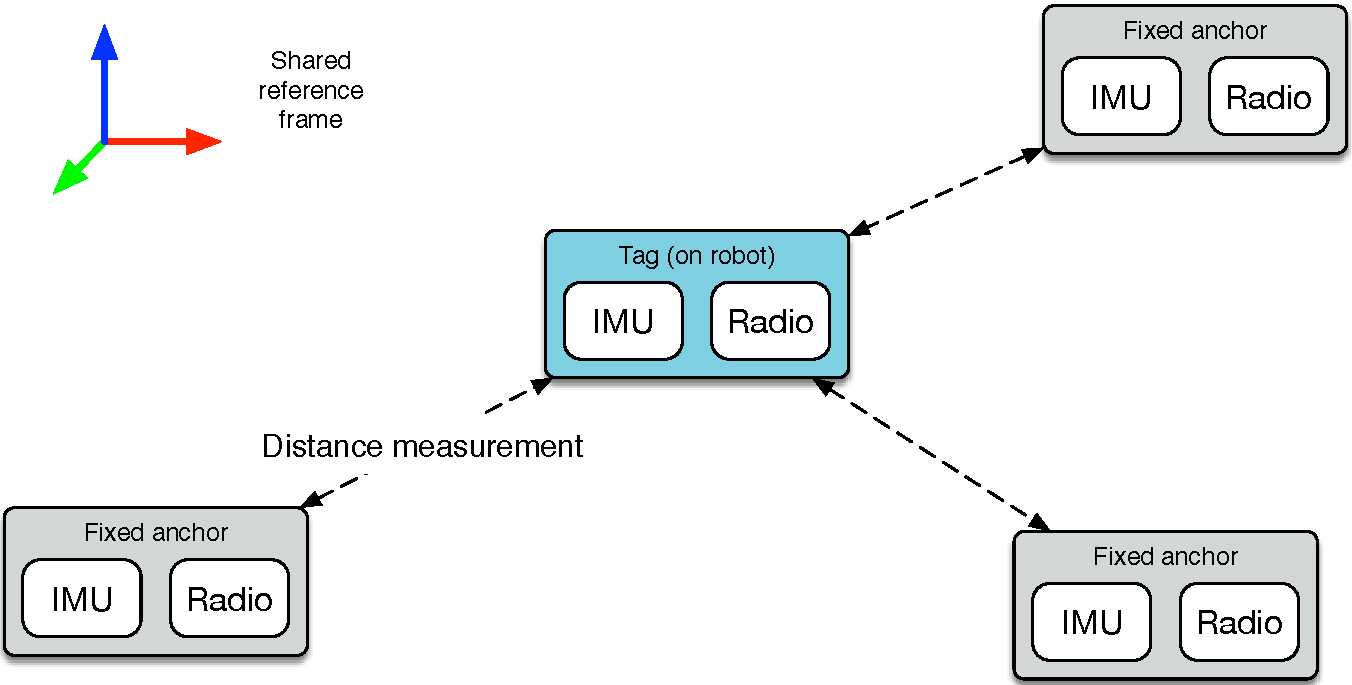
\includegraphics[width=\textwidth]{figures/system.pdf}
    \caption{Overview of the system, showing one mobile robot (blue) and three fixed anchors (grey).}
    \label{fig:system}
\end{figure}

The complete system (Figure~\ref{fig:system}) is made of two types of nodes, tags and anchors.
The distance between each node is obtained by measuring the time of flight for a radio packet.
The tags are placed on each robot, and estimate their position using the \gls{imu} combined with the distance measurements to the anchors.
The anchors are at a reference position (fixed) and can be used by several tags.
A tag will always use all the available tags and will be able to seamlessly switch in case a tag is not in range anymore.

\section{Tasks}

After doing a review of the literature on the topic, I will start by doing a model of the system.
This includes both the dynamics of the system and the impact of noise on precision.
I should also investigate if the Digital Motion Processing unit built in the \gls{imu} can be useful.
I will then develop a position estimator taking the \gls{imu} data as inputs and the distance readings as measurements.

In parallel to this, I will write code for the reference board (Figure~\ref{fig:board}).
Several steps must be done in order to have a working system:
\begin{inparaenum}
    \item Drivers for the \gls{uwb} module and the \gls{imu} chip.
    \item Distance measurement protocol.
    \item Position estimation algorithm.
\end{inparaenum}

I will finish my work by measuring the performance of the system.
If time remains, I would like to implement a protocol to communicate over the \gls{uwb} link, to provide low bandwidth inter-robot communications without additional hardware.

\begin{figure}[h!]
    \centering
    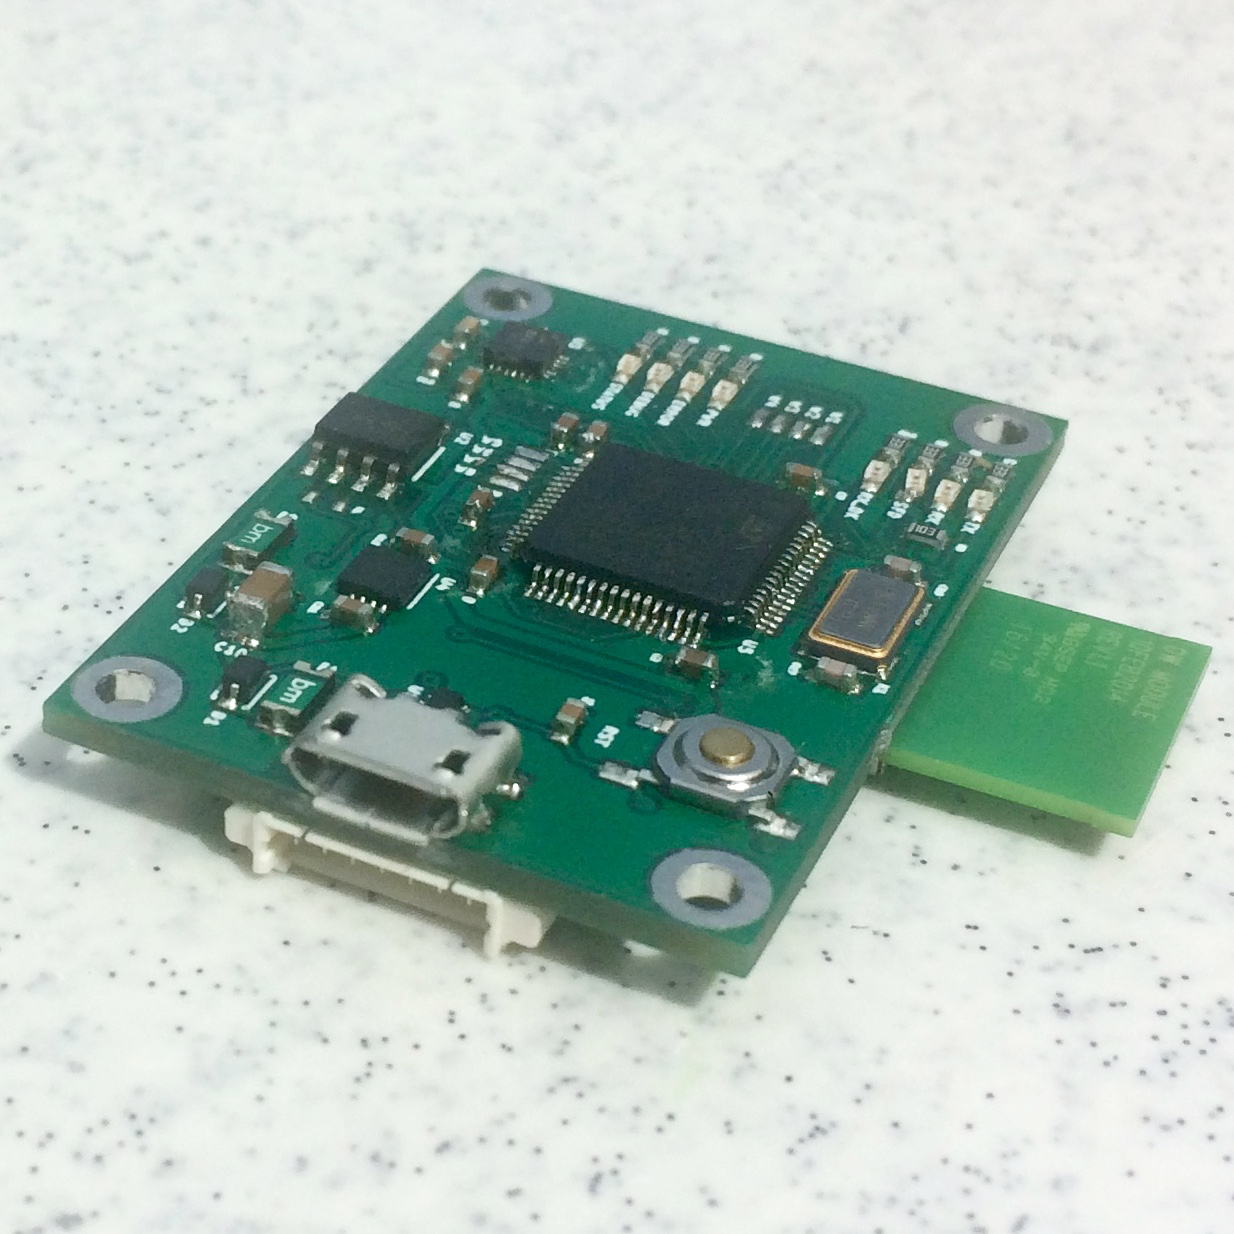
\includegraphics[width=0.4\textwidth]{figures/board}
    \caption{Reference board which includes an STM32F405 processor, a DWM1000 \gls{uwb} module and an MPU9250 \gls{imu}.}
    \label{fig:board}
\end{figure}

\section{Expected results}

\begin{enumerate}
    \item Working system.
        The tags should be able to estimate their position correctly and stream it to a laptop via USB or CAN.
        They should also be easy to configure for another anchor setup.
    \item Performance characteristics.
        I would like to measure the error distribution of the estimated position and compare those to theoretical optimums to ensure the system is well working.
        I will also measure the impact of anchor placement on performance.
\end{enumerate}

\end{document}

\end{abstract}

\end{center}
\end{titlepage}

\section{Mechanical design and locomotion system}
250 word + image

images/rover-front.png
images/rover-side.png
images/rover-top.png

\begin{figure}[htbp]
   \caption{\label{fig:rover} CAD view of the rover}
   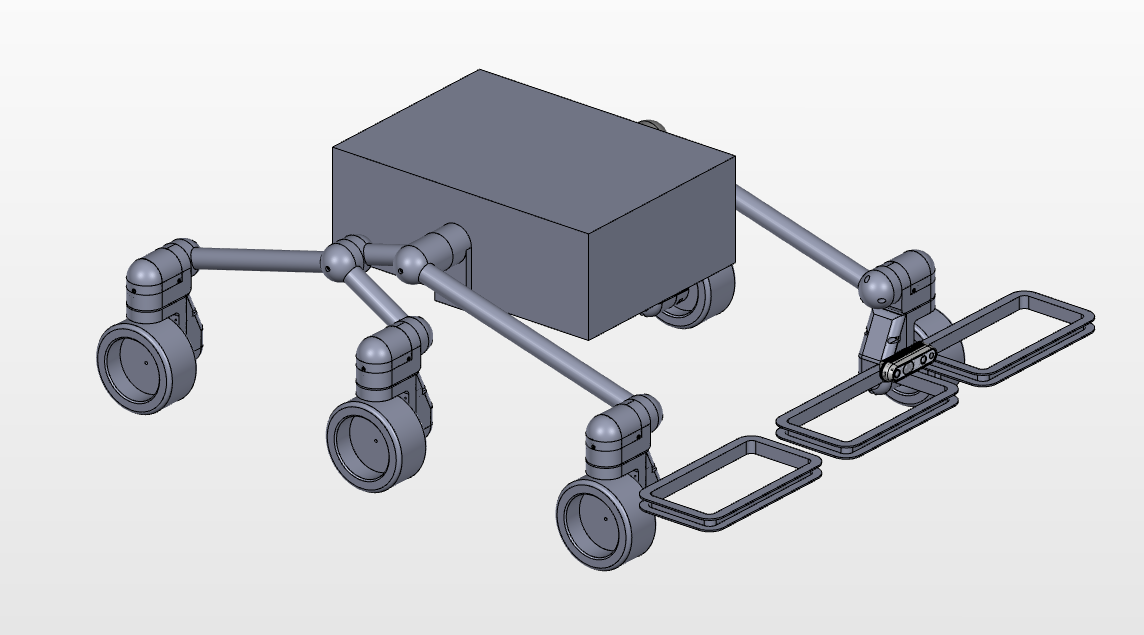
\includegraphics[width=\textwidth]{images/rover}
\end{figure}

\section{Sensors and landmine detection}
We detect landmines through two sensor measurements:
\begin{enumerate}
    \item a pulse induction metal detector to detect surface and buried landmines
    \item an RGBD sensor to detect surface landmines
\end{enumerate}

The metal detector is built around a resistor-inductor circuit formed by the coil.
We charge this coil with short pulses in the range of its characteristic time-constant $\tau = \frac{L}{R}$.
Then we measure the discharge signal and fit an exponential curve to it.
Three cases can arise:
\begin{enumerate}
    \item Nothing is observed, hence we only observe $\tau$ of the coil
    \item Non-ferromagnetic metal is near, hence we observe a shorter $\tau$ on the discharge curve because the eddy currents generated in the metal by electromagnetic stimulation decay the magnetic field faster
    \item Ferromagnetic metal is near, hence we observe a longer $\tau$ on the discharge curve because the ferromagnetic metal will be magnetized temporarily and retains the magnetic field longer
\end{enumerate}
In order to make this detection more reliable, we had to compensate for temperature drift on the measurement.
Driving the coil at high power heats it, which makes the resistance grow as $R = R_0 (1 + a T + a T^2)$.

A complementary detection mechanism is implemented using an RGBD sensor.
From the sensor data we build a local point cloud of the scene in front of the rover.
Then, we segment it to extract objects from the ground.
Objects that fit the geometric and color description of a landmine are logged.

\section{Electronic circuit and control system}
250 words + image

\section{Area navigation}
Our navigation is simple but open for extension.
The rover will be manually driven, however everything is such that the onboard computer could control the rover.
The idea is the cover the field in a grid pattern, while going around any landmines we encounter.

\section{Mapping}

To map the competition area, our robot will use a custom localization system that we developped.
Similarly to GPS, our system computes the rover's position by using the \gls{rtt} of a radio signal to several fixed beacons, of which the position is known.

We use Decawave's DWM1000 radio modem with a custom protocol to measure the distance.
This gives us a good distance measurement accuracy: $1 \sigma = \SI{3}{\centi\meter}$.

Since we know the distance to each fixed beacons, as well as their positions, we can compute the position of the robot.
This is done using an \gls{ekf}, using the distance to a point as a correction function.
For the prediction step, we originally planned to use an inexpensive \gls{imu}, similar to the ones found in mobile phones.
However we probably won't implement it, due to time constraints.

The system was already tested on a \SI{20}{\meter} by \SI{20}{\meter} open field at our workshop.
We got very good positioning results and reliability, although we lacked time to do a quantitative analysis of the measurement accuracy and precision.
According to simulation, we should be within \SI{10}{\centi\meter} of ground truth.
As the reliability so far is good, we will be using this system only for Minesweepers 2018.


\section{Rough environment handling}

250 words

\textbf{YOUTUBE VIDEO}


\clearpage
\appendix

\clearpage
\nocite{*} % tells bibtex to include everything
\bibliographystyle{chicago}
\bibliography{report}

\end{document}
